
\subsection{Geometric structure}

We begin with some geometric generalities; for more details, see the monograph of Tao \cite[Chapter 6.2]{Tao2006} and the notes of Tataru \cite[Geometric Dispersive Equations]{KochEtAl2014}.  Given a map $u : I \times \R^2 \to \SS^2$, we will use $\bfD_j$ to denote the pullback of the connection on the sphere, and $\bfJ$ the complex structure given by $\tfrac\pi2$-rotation. Using this notation, the equation \eqref{schrodinger} takes the form
\begin{equation}\label{eq:geoschrod}
        \partial_t u 
            = \bfJ (\bfD_1 \partial_1 u + \bfD_2 \partial_2 u).
\end{equation}


To reveal the linear Schr\"odinger structure of the equation, it is convenient to fix an orthonormal frame $\{\vec v, \vec w\} \subseteq u^* T\SS^2$ on the pullback bundle. Using this frame, we can identify each tangent space $T_{u(t, x)} \SS^2$ with $\C$ via the isomorphism 
    \begin{align*}
        T_{u(t, x)} \SS^2
            &\longrightarrow \C, \\
        X^1 \vec v + X^2 \vec w 
            &\longmapsto X^1 + i X^2.        
    \end{align*}
Thus we can identify the field $v : I \times \R^2 \to u^* T\SS^2$ with a complex scalar field $\psi: I \times \R^2 \to \C$, 
    \[
        \psi 
            := \big\langle v, \vec v \big\rangle \, \vec v + i \big\langle v, \vec w \big\rangle \, \vec w.
    \]
In particular, we will denote $\psi_\alpha$ for the differentiated fields $\partial_\alpha u$. In this frame, the action of the covariant derivative on the field $v$ corresponds to the following operation on the complex scalar field $\psi$, 
    \[
        \bfD_\alpha v 
            \longmapsto (\partial_\alpha + i A_\alpha) \psi, 
    \]
where the frame coefficients $A_\alpha := \langle \bfe_2, \partial_\alpha \bfe_1 \rangle$ track the change in the frame $\{\bfe_1, \bfe_2\}$ relative to the vector field $\partial_\alpha$. We abuse notation by denoting the operator on the right by $\bfD_\alpha \psi$. \textit{A priori}, the connection coefficients satisfy the curl system 
    \begin{equation}\label{eq:curvature}
        \partial_\alpha A_\beta - \partial_\beta A_\alpha 
            = \Im (\psi_\alpha \overline{\psi_\beta}),
    \end{equation}

Note that thus far we have not fixed a frame; indeed, any other frame could be obtained from rotating by $e^{i \chi}$. Varying the gauge choice leads to the gauge invariance
    \[
        \psi \mapsto e^{i \chi} \psi, \qquad A_\alpha \mapsto A_\alpha + \partial_\alpha \chi. 
    \]
Fixing a gauge fully determines the connection coefficients in terms of the original field $u$. We will work with Coulomb gauge, 
    \begin{equation}\label{eq:coulomb}
        \partial_1 A_1 + \partial_2 A_2 = 0,
    \end{equation}
which, upon differentiating the curvature relation \eqref{curvature} and inverting the Laplacian, we see that the connection coefficients are given precisely by 
    \begin{equation}\label{eq:coefficients}
        A_\alpha [\psi] 
            = -\frac12 \Delta^{-1} \partial^\beta \Im(\psi_\alpha \overline{\psi_\beta}). 
    \end{equation}
In general, this has unfavourable high $\times$ high $\to$ low interactions, as schematically the right-hand side takes the form $D^{-1} (\psi \overline \psi)$, though in our setting of equivariant symmetry, the situation is much better. In any case, thinking of the connection coefficients as quadratic terms, we can rewrite the Hasimoto-transformed system \eqref{hasimoto} in these coordinates as the cubic-type non-linear Schr\"odinger equation 
    \begin{equation}
        i\partial_t \psi_{\overline z} - \Delta \psi_{\overline z} 
            = A_t [\psi] \psi_{\overline z} + i \partial_{\overline z} A_z[\psi] \psi_{\overline z} + i A_z [\psi] \partial_{\overline z} \psi_{\overline z} + i A_{\overline z} [\psi] \partial_z \psi_{\overline z} - A_z [\psi] A_{\overline z}[\psi] \psi_{\overline z}. 
    \end{equation}



\begin{figure}[h]
    \begin{center}
        \begin{tikzcd}
            (I \times \R^2) \times \C \arrow[r, "\bfe"] & u^* T \SS^2 \arrow[d, "v"] \arrow[r, "u"] & T\SS^2 \arrow[d] \\
            I \times \R^2 \arrow[u, "\psi"'] \arrow[r]  & I \times \R^2 \arrow[r, "u"]                        & \SS^2           
            \end{tikzcd}
            \caption{The commutative diagram connecting the trivial bundle $(I \times \R^2) \times \C$, the pullback bundle $u^* T\SS^2$, and the tangent bundle $T\SS^2$. }
    \end{center}
\end{figure}



\begin{proposition}[Schr\"odinger maps in Coulomb gauge]
    Let $m \in \N$ and $\bfm$ be a solution to Landau-Lifshitz. Then the equation in Coulomb gauge     
\end{proposition}


\subsection{Splitting and orthogonality}

To identify our enemies, let us detail the derivation of the linearised equation \eqref{linearised}. Starting from decomposition of the solution into soliton profile and error \eqref{decomp2}, we further decompose the error into a component perpindicular to the soliton (i.e. in the tangent space $T_Q \SS^2$) and a component parallel to the soliton,
    \begin{equation}
        \begin{split}
            u(t, r) 
                &=  \underbrace{Q(r)}_{\text{soliton profile}} + \underbrace{\epsilon(t, r)}_{\text{perturbation}} \\
                &= \underbrace{Q(r)}_{\text{soliton profile}} + \underbrace{u_{\mathrm{lin}} (t, r)}_{\text{perpindicular perturbation}} + \underbrace{\gamma(t, r) Q(r)}_{\text{parallel perturbation}}
        \end{split}
    \end{equation}
For small perturbation $|\epsilon| \ll 1$, the main term is the perpindicular component in view of the constraint $|u| \equiv |Q| \equiv 1$; indeed one can compute that the parallel component is of quadratic order, 
    \[
        \gamma = \sqrt{1 - |u_{\mathrm{lin}}|^2} - 1 = O(|u_{\mathrm{lin}}|^2). 
    \]


\begin{figure}[h]
    \begin{center}
        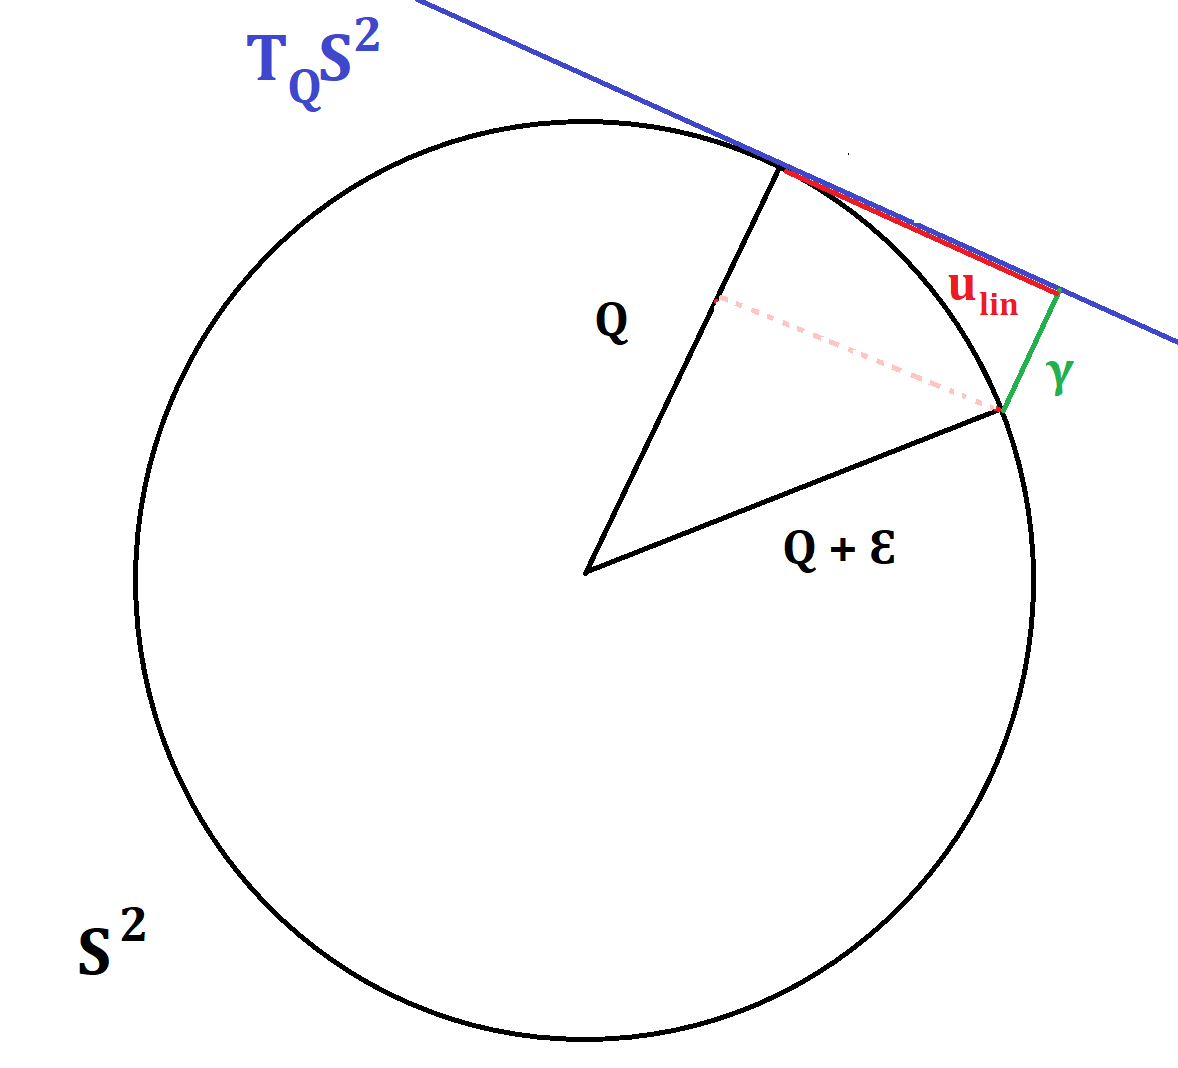
\includegraphics[scale = 0.3]{graphics/coulombQ}
        \caption{Decomposition of the solution 
            \[u = Q + (u_{\mathrm{lin}} + \gamma),\] 
        into a component parallel to the soliton $\gamma \in \operatorname{span} Q$ and a component in the tangent space $u_{\mathrm{lin}} \in T_Q \SS^2$. }
    \end{center}
\end{figure}

The Coulomb frame 
    \[
        \vec v_Q (r) 
            = \begin{pmatrix} h_3 (r) \\ 0 \\ - h_1 (r) \end{pmatrix},
        \qquad
        \vec w_Q (r) 
            = \begin{pmatrix} 0 \\ 1 \\ 0 \end{pmatrix}. 
    \]